\documentclass[11pt,compress,t,notes=noshow, aspectratio=169, xcolor=table]{beamer}

\usepackage{../../style/lmu-lecture}
% Defines macros and environments
% This file is included in slides and exercises

% Rarely used fontstyle for R packages, used only in 
% - forests/slides-forests-benchmark.tex
% - exercises/single-exercises/methods_l_1.Rnw
% - slides/cart/attic/slides_extra_trees.Rnw
\newcommand{\pkg}[1]{{\fontseries{b}\selectfont #1}}

% Spacing helpers, used often (mostly in exercises for \dlz)
\newcommand{\lz}{\vspace{0.5cm}} % vertical space (used often in slides)
\newcommand{\dlz}{\vspace{1cm}}  % double vertical space (used often in exercises, never in slides)
\newcommand{\oneliner}[1] % Oneliner for important statements, used e.g. in iml, algods
{\begin{block}{}\begin{center}\begin{Large}#1\end{Large}\end{center}\end{block}}

% Don't know if this is used or needed, remove?
% textcolor that works in mathmode
% https://tex.stackexchange.com/a/261480
% Used e.g. in forests/slides-forests-bagging.tex
% [...] \textcolor{blue}{\tfrac{1}{M}\sum^M_{m} [...]
% \makeatletter
% \renewcommand*{\@textcolor}[3]{%
%   \protect\leavevmode
%   \begingroup
%     \color#1{#2}#3%
%   \endgroup
% }
% \makeatother

\newcommand{\open}{}
\newcommand{\close}{}

\title{Interpretable Machine Learning}
% \author{LMU}
%\institute{\href{https://compstat-lmu.github.io/lecture_iml/}{compstat-lmu.github.io/lecture\_iml}}
\date{}

\begin{document}

\newcommand{\titlefigure}{figure/25-05-31_Hooker_2004_graph_fANOVA}
\newcommand{\learninggoals}{
\item Limitations of classical fANOVA
\item Alternatives: Generalized fANOVA and ALE
% \item Overcoming these limitations with generalized fANOVA
% \item How ALE Plots can be used as another, different approach to obtain functional decompositions
% \item Sobol-Hoeffding decomposition ??
\item Advantages and relevance of functional decompositions
}

\lecturechapter{Functional Decompositions: Further Methods}
\lecture{Interpretable Machine Learning}

\begin{frame}{Limitations of classical fANOVA}

    \begin{itemize}
    
        \item Standard fANOVA builds on PD-functions
        
        \item \textit{Remember:} Problems of PDPs for \textbf{correlated / dependent features}
        \item Here: Dependent features $\implies$ Standard fANOVA does NOT fulfill vanishing conditions %(Similar problem also for H-statistic, although may still offer some insight)
    \end{itemize}
    \pause
    \begin{example}
        Assume dependency \(2x_1^2 = x_2\) and
        \begin{equation*}
            \fh(x_1, x_2, x_3) = - 2x_1 - 2\sin(x_3) + |x_1|x_2 + 0.5 x_2 x_3 + 1.
        \end{equation*}
        % $$
        % \fh(x_1, x_2, x_3) = - 2x_1 - 2\sin(x_3) + |x_1|x_2 + 0.5 x_1 x_2 x_3 - \sin(x_2 x_3) + 1
        % $$
        $\leadsto$ Following two decompositions would both ``make sense'':
        \begin{align*}
            \fh(x_1, x_2, x_3)
            = \underbrace{1}_{g_\emptyset}
                + \underbrace{(- 2x_1)}_{g_1(x_1)} 
                + \underbrace{(- 2\sin(x_3))}_{g_3(x_3)}
                + \underbrace{|x_1|x_2}_{g_{1,2}(x_1, x_2)} 
                + \underbrace{0.5 x_2 x_3}_{g_{2,3}(x_2, x_3)} \\
            \fh(x_1, x_2, x_3)
            = \underbrace{1}_{g_\emptyset}
                + \underbrace{(- 2x_1 + 2 |x_1|^3)}_{g_1(x_1)} 
                + \underbrace{(- 2\sin(x_3))}_{g_3(x_3)}
                + \underbrace{x_1^2 x_3}_{g_{2,3}(x_1, x_3)}
        \end{align*}
    \end{example}
    \pause
    $\rightarrow$ Extreme example, but again: Problem of definition

    % [Example going wrong with correlated features]

    
    
\end{frame}

\begin{frame}{Alternative: Generalized Functional ANOVA}

\begin{itemize}
    \item Algorithm proposed by \citebutton{Hooker (2007)}{http://www.tandfonline.com/doi/abs/10.1198/106186007X237892}
    \item Generalizes standard fANOVA to situations with dependent features
    \pause
    \item Showed: Generalized fANOVA is solution to so-called ``relaxed vanishing conditions'' \\
    (i.e., weaker form of vanishing condition) \\
    \item ``Relaxed vanishing conditions'' do not imply orthogonality, but ``hierarchical orthogonality'':
    $$
    \mathbb{E}_{\Xv} \bigl[ g_{V}(\xv_V) g_{S}(\xv_S) \bigr] = 0 \quad \forall V \subsetneqq S
    $$
    \pause
    $\leadsto$ Only components are orthogonal where $g_{V}(\xv_V)$ is ``lower in hierarchy'' than $g_{S}(\xv_S)$
    \item[$\implies$] Generalized fANOVA provides functional decomposition for arbitrary settings
    \item \textbf{Advantage:} Also provides a variance decomposition
    \pause
    \item \textbf{Problems:}
    \item Difficult to estimate, involves manual choice of a ``weight function''
    \item Computationally very costly
    
\end{itemize}

    % \textbf{N.B.:} For dependent inputs, \citebutton{Hooker (2007)}{http://www.tandfonline.com/doi/abs/10.1198/106186007X237892} showed the existence of a unique solution for the components under a ``relaxed vanishing condition'' which leads to a ``hierarchical orthogonality''
    % $$\mathbb{E}_{\Xv} (g_{V}(\xv_V) g_{S}(\xv_S)) = 0, \forall V \subsetneqq S$$
    % $\leadsto$ Only components are orthogonal where features involved in $g_{V}(\xv_V)$ also appear in $g_{S}(\xv_S)$
    % Only components where all features involved in one component $g_{V}(\xv_V)$ also appear in the other component $g_{S}(\xv_S)$ are orthogonal

    % \pause

    % \textit{[Also talk about constraints corresponding to generalized fANOVA ?]}
    
\end{frame}

% \begin{frame}{Generalized fANOVA: Example}

%     Example from above ??
    
% \end{frame}

\begin{frame}{Revisiting ALE Plots}

    \[
    \hat{\tilde{f}}_{S, ALE}(x) = \sum_{k = 1}^{k_S(x)}\frac{1}{n_S(k)}\sum_{i: \; x_S^{(i)} \in \; [z_{k-1, S}, z_{k, S}]}\left[\fh(z_{k, S}, \xi_{-S}) -\fh(z_{k-1, S}, \xi_{-S})\right]
    \]

    \begin{columns}[c, totalwidth=\linewidth]
    \begin{column}{0.5\textwidth}
        % 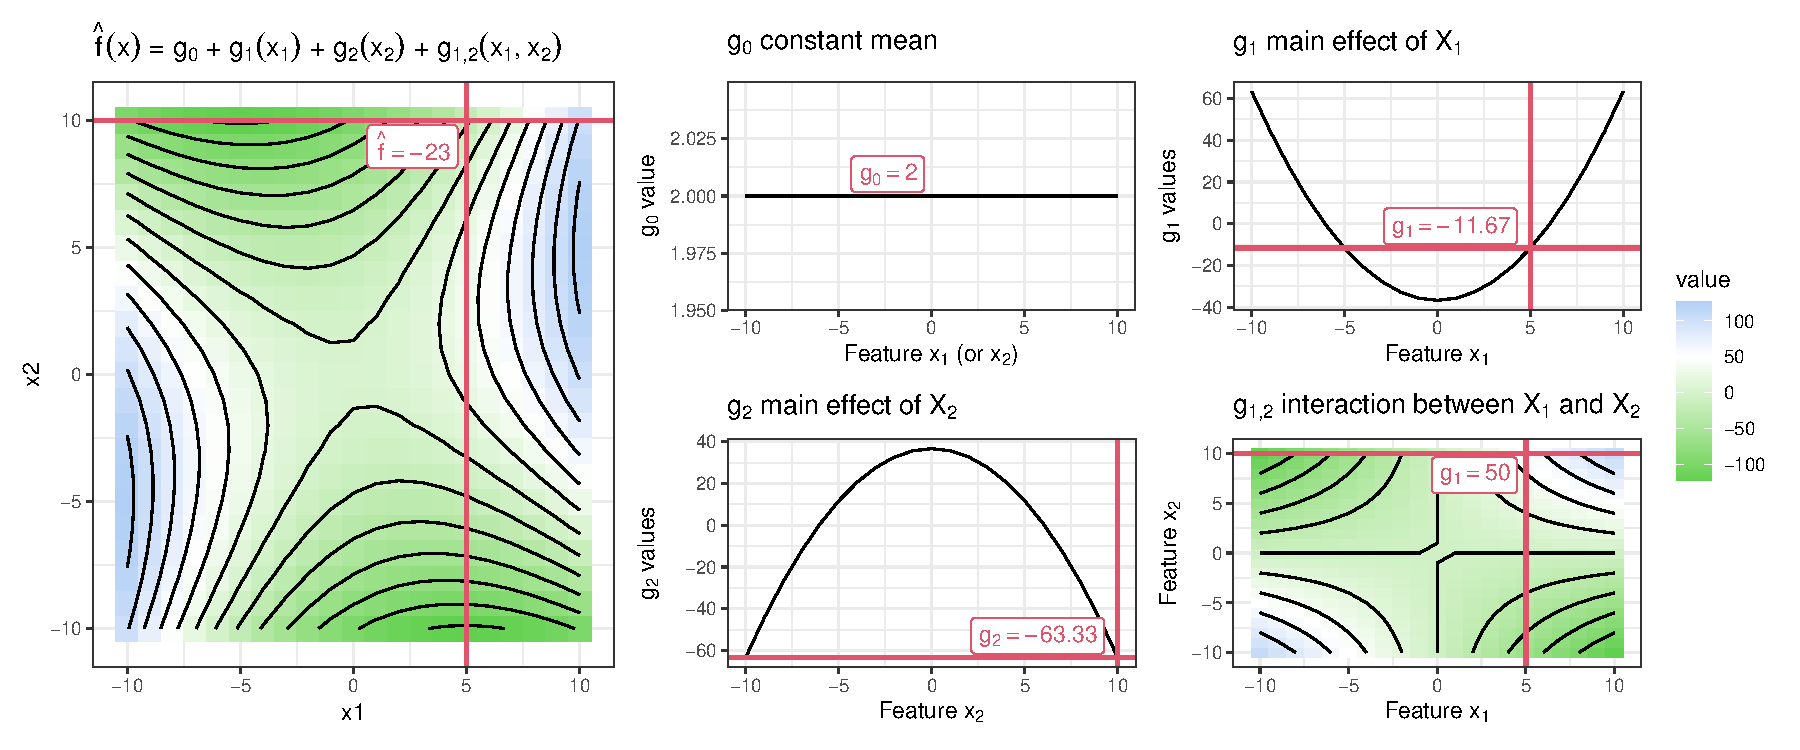
\includegraphics[width = \textwidth]{figure/decomposition}
        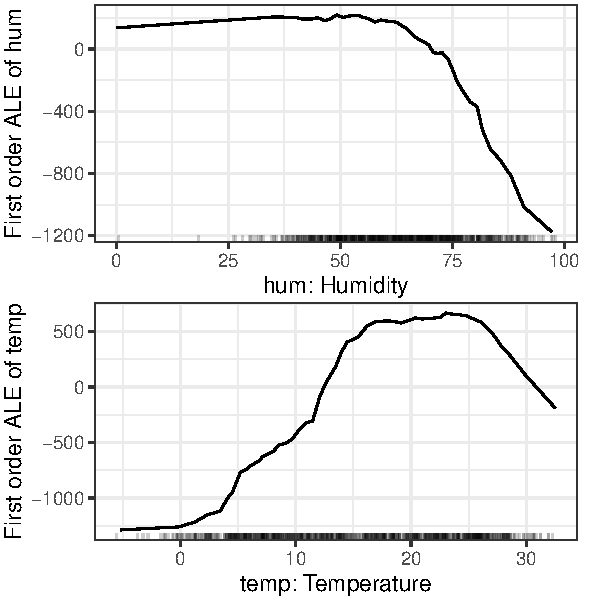
\includegraphics{figure/ale1d}
    \end{column}
    \begin{column}{0.5\textwidth}
        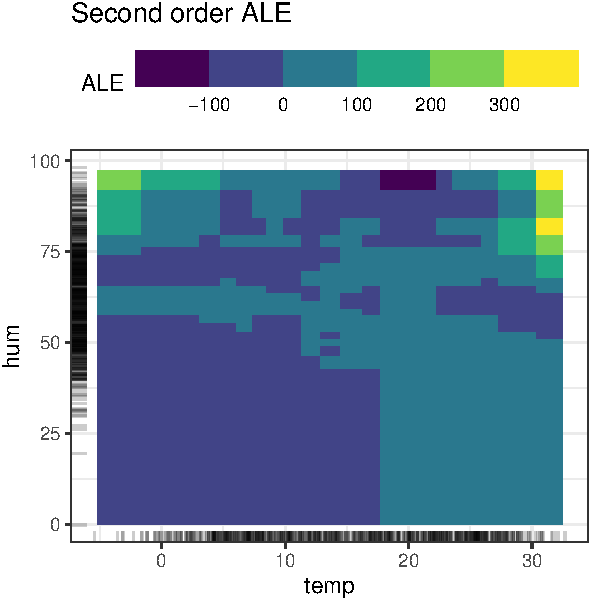
\includegraphics{figure/ale2d}
    \end{column}
    \end{columns}

    % \splitV{
        % \image{figure/ale1d}
    % }{
        % \image{figure/ale2d}
    % }
    
\end{frame}

\begin{frame}{ALE Decomposition}

    \begin{itemize}
        \item One can define ALE plots for arbitrary many variables \\
        (similar to PDPs vs. PD-functions)
        \item[$\rightarrow$] Gives full functional decomposition of ALE plots
        \pause
        \item \textbf{Advantages:} Handle dependencies well + computationally fast
        \item Constraints / orthogonality properties more complicated
        \item[$\implies$] ALE decomposition theoretically more involved, but good alternative in practice
    \end{itemize}
    
\end{frame}

% \begin{frame}{Sobol-Hoeffding decomposition}
    
% \end{frame}

% \begin{frame}{if enough time: Constraints (theory) for these other methods}

%     NB: Even more possible constraints (leading to ever more different decompositions) have been developed in research papers.
    
% \end{frame}

\begin{frame}{Conclusion: How useful are functional decompositions?}

    % Obwohl fDecompositions eigtl (aus Interpretability-Sicht) die Lösung für alles wären / theoretisch die Endlösung sind, sind alle anderen Methoden trotzdem nötig, weil fDecompositions sehr schwierig \& kompliziert zu berechnen sind
    % - Computation time skaliert exponentiell mit der Dimension / Anzahl features  =>  i.a. ist Erzwingen einer sparsen decomposition (s. GAMs / RPFs) die einzige realisitische Möglichkeit

    \begin{itemize}
        
        \item If computed, offer a lot of insight into a model or function, i.p. high-dimensional
        \item[$\rightarrow$] Complete analysis of all interactions
        \pause
        \item Very important theoretical concept:
        \begin{itemize}
            \item Theoretical framework for general definition of interactions (H-statistic)
            \item Theoretical background for many IML methods:
                GAMs and EBMs, 
                ICE, PDPs and PD-functions,
                ALE plots,
                Shapley values,
                Feature importance methods (see later)
            % \item GAMs and EBMs
            % \item ICE, PDPs and PD-functions
            % \item ALE plots
            % \item Shapley values (see later)
            % \item Feature importance methods (see later)
        \end{itemize}
        \pause
        \item In practice often infeasible ($2^p$ components for $p$ features)
        \item[$\implies$] Often only sparse decompositions feasible (E.g. EBMs)
        \pause
        \item All single methods have disadvantages:
        \begin{itemize}
            \item Standard fANOVA: Only independent features + compute intensive
            \item Generalized fANOVA: Even more compute intensive, evtl. infeasible
            \item ALE: No variance decomposition
        \end{itemize}
        
    \end{itemize}

    \pause
    % Nevertheless, functional decompositions are a very important concept in machine learning interpretability because they explain the idea behind many other methods and enable a much better understanding of other methods.
    \textbf{Overall:} Very important concept and theoretical background, explains idea behind many other methods
    
\end{frame}










\endlecture
\end{document}
